\section{APPENDIX}


\begin{figure}[h]
    \centering
    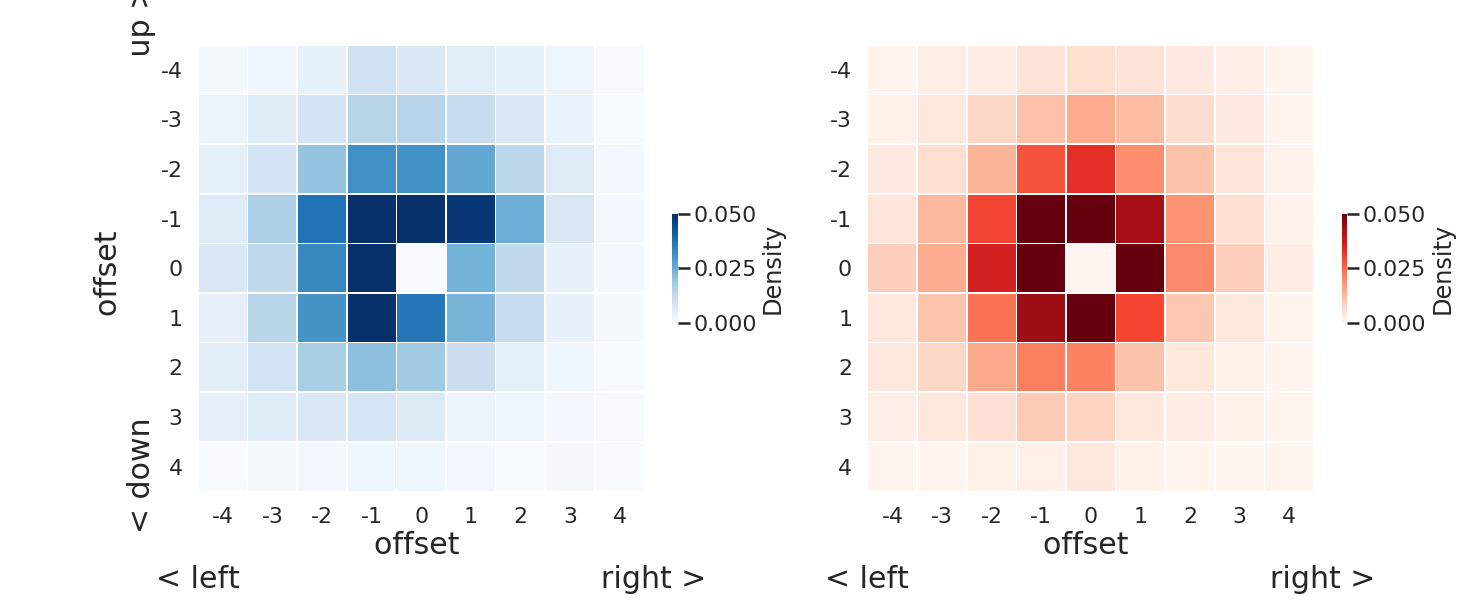
\includegraphics[scale=0.25]{source/figures/results/shelf_grasp_offsets.png}
    \caption[]{Object displacement behavior for the two task types. The left panel (blue heatmap) shows the movement offset for the EASY trials, right panel (red heatmap) for HARD trials. The movement offset is defined as the difference of the row-wise and column-wise difference of the drop-off location and pickup location at the end and beginning of the action execution respectively. Negative numbers in the ordinate refer to the object movement being upward and negative numbers in the abscissa refer to object displacement being leftward. For the EASY trials, most objects are moved one row upward and one column leftward. For the HARD trials, the object movement is also upward and leftward. For both trials, a majority of the final location is in the immediate vicinity of the initial location of the object.}
    \label{figure:offset}
\end{figure}


\begin{figure}[h]
    \centering
    \subfloat[]{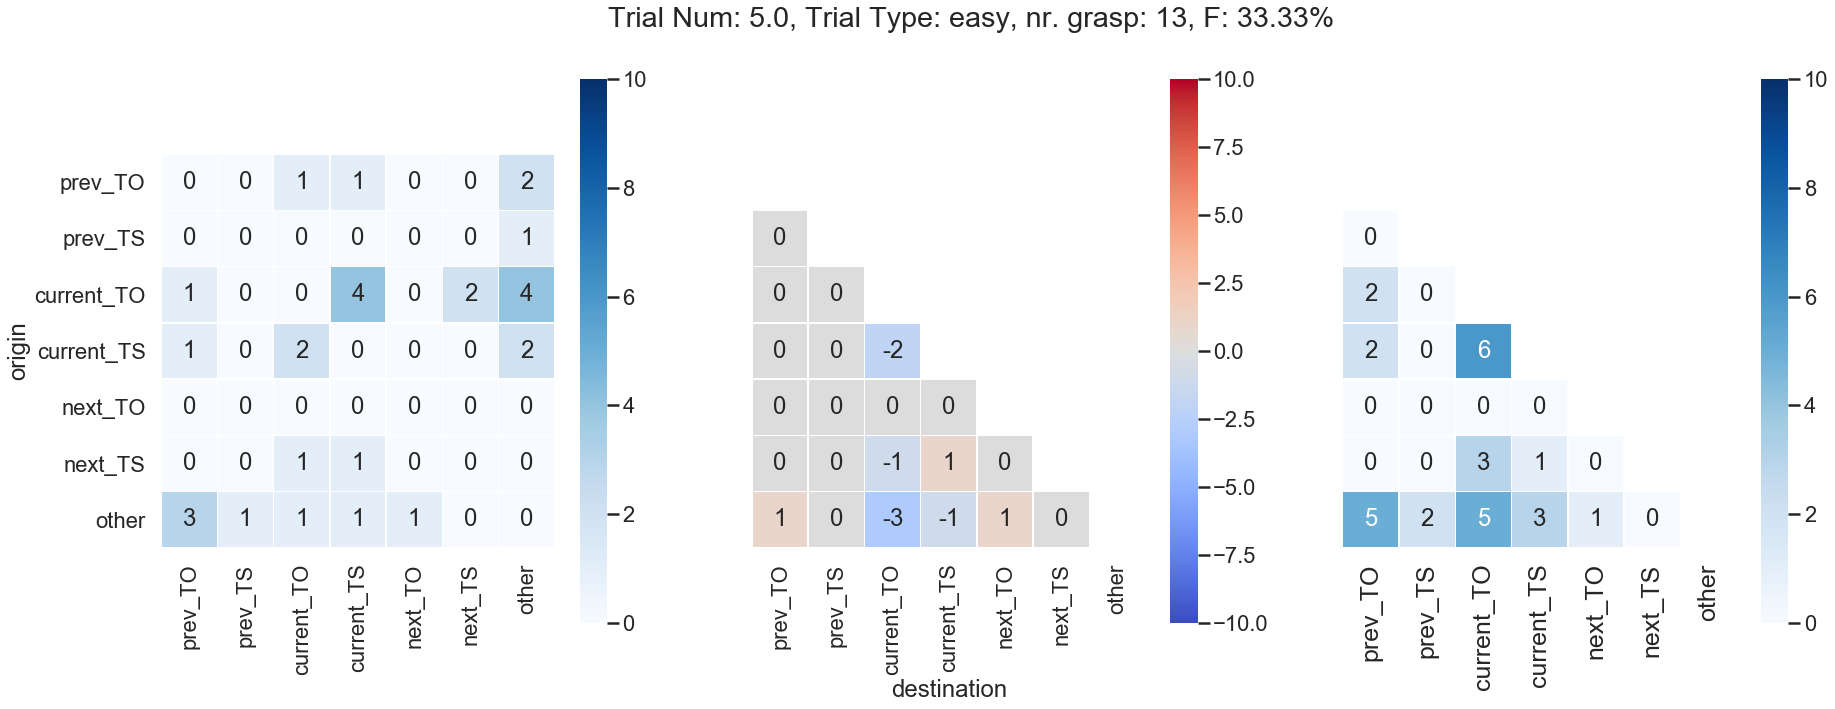
\includegraphics[width=0.7\linewidth]{source/figures/results/transition_matrix_trial_5_exe.png}
    \label{figure:transition_1}} \\
    \subfloat[]{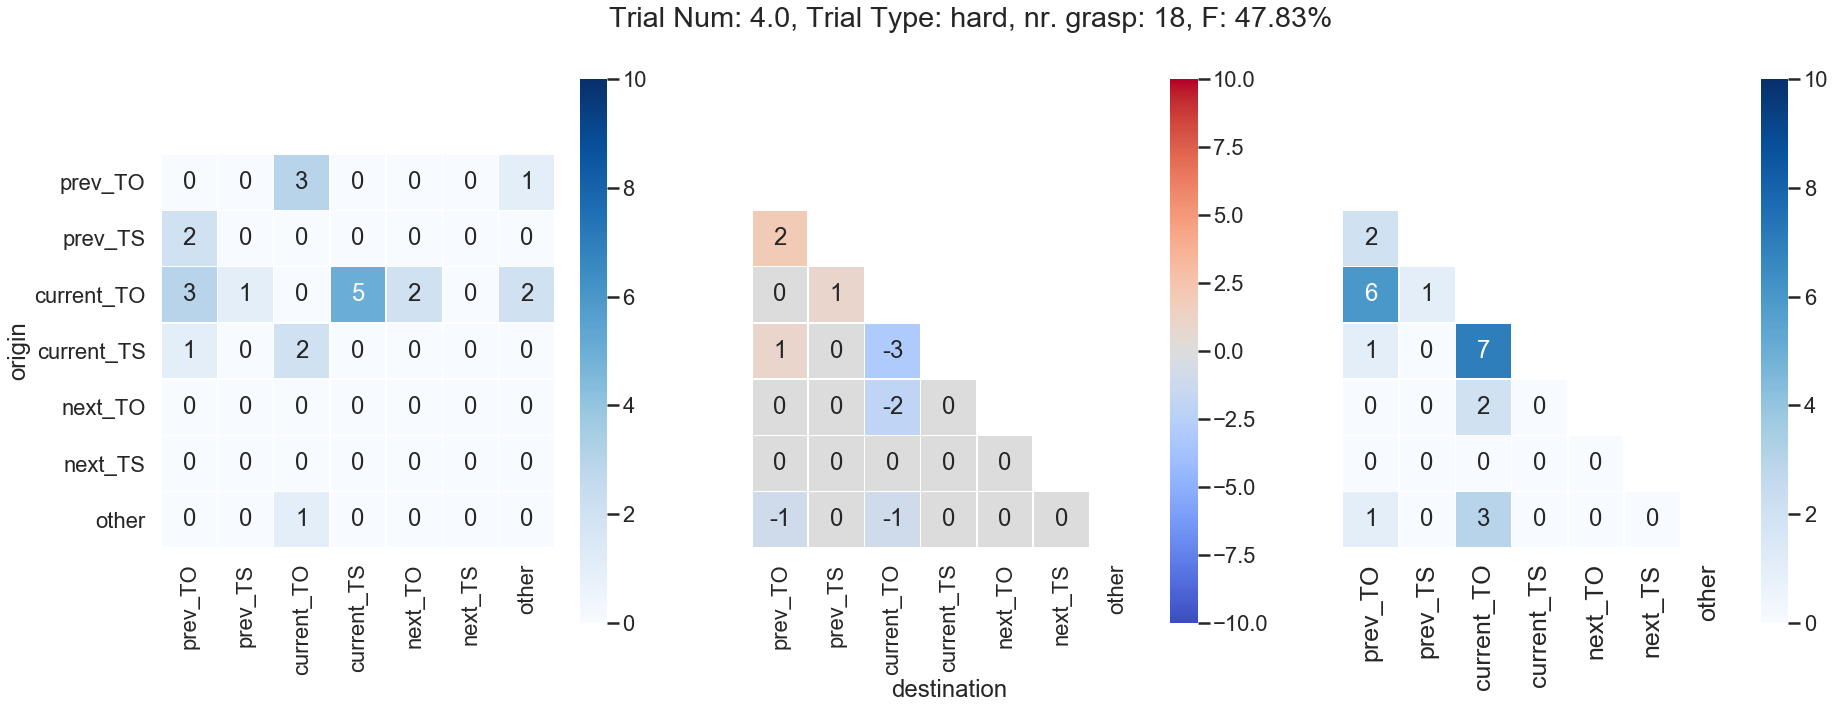
\includegraphics[width=0.7\linewidth]{source/figures/results/transition_matrix_trial_4_exe.png}
    \label{figure:transition_2}}
    \caption[]{Exemplar transition matrices for gaze switching between end of previous grasp and start of current grasp for the two trial types. The ordinate denotes the origin of the gaze i.e. where the gaze was before and the abscissa denotes the destination of the gaze. The diagonal contains zero as the transition is defined as a saccade from one ROI to another and not re-fixations on the same ROI. The left panel shows the transition matrix, A. The middle panel, shows the net transitions (A\textsubscript{NET}) The positive number in the matrix denotes transitions from source ROI to destination ROI, whereas the negative numbers reverse the direction of transition. The right panel shows the total transitions (A\textsubscript{TOTAL})  made between the 7 regions of interest. The F-value in the in the figure title refers to the relative number of net transitions compared to total transition matrix along with the the number of grasps and the trial type.  \\
    Panel \protect\subref{figure:transition_1} shows the transition matrix for gaze switching in an EASY trial with 13 grasps/object displacements. As shown in the middle panel, in the trial, there is 1 net transition are made to prev\_TO to other, whereas 3 transitions are made from current\_TO to 'other'. The right panel shows the total number of transitions made between the the ROIs. This tells us the that a majority of the transitions are from 'other' sources to the regions of interest. The F value for this trial shows that 33.33\%  net transitions are present in the total transitions.\\
    Panel \protect\subref{figure:transition_2} shows the transition matrix for gaze switching of in a HARD trial with 18 grasps/object displacements. As shown in the middle panel, in the trial, 8 transitions are made from prev\_TO to other, and 8 transitions are made from 'other' to current\_TO. And other ROI have close to net zero transitions. The right panel shows the total number of transitions made between the the ROIs. It tells us the that a majority of the transitions are from current\_TO to the current\_TS. The F-value for this trial shows that 47.83\%  net transitions are present in the total transitions.}
    \label{figure:transition_matrices_exe}
\end{figure}

\begin{figure}[h]
    \centering
    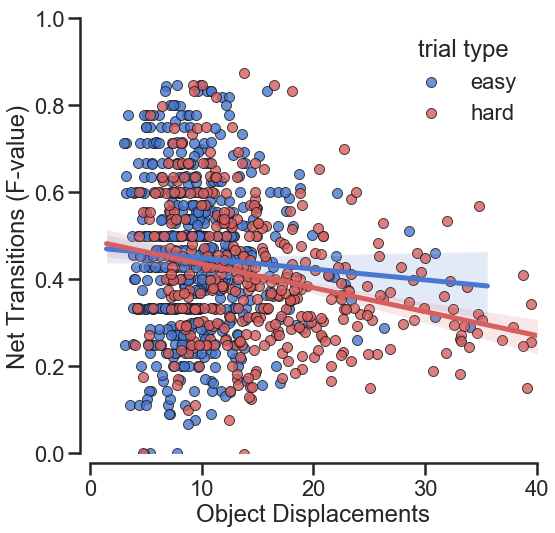
\includegraphics[width=0.3\linewidth]{source/figures/results/gaze_guidance_v_grasps_execution.png}
    \caption[]{Gaze guidance behavior vs. number of object displacements. Figure shows a scatter plot of the relative net transition (F-value) vs. number of object displacements per trial and subject differentiated the two trial types EASY(blue), HARD(red). Each point refers to one trial and it's F value vs. the number of object displacements in that trial. The lines denote the regression fit and the shaded region denotes 95\% confidence interval. F-values for both trial types decrease with increasing number of object displacements. Specifically, higher number of object displacements in a trial is correlated with lower gaze guidance. Pearson correlation $\rho$= -0.05 (p = 0.16) for EASY trials and $\rho$ = -0.25 (p<0.000) for HARD trials.}
    \label{figure:F_value_exe}
\end{figure}

\begin{figure}[]
    \centering
    \subfloat[]{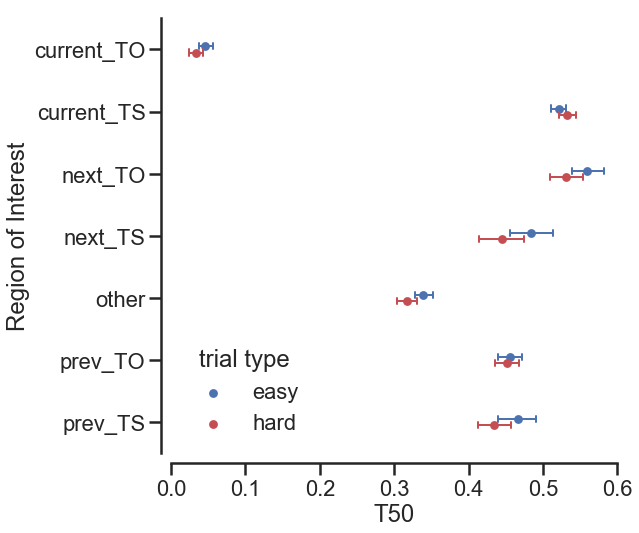
\includegraphics[width=0.3\linewidth]{source/figures/results/t50_subject_execution.png}\label{figure:t50_sub_exe}}
    \subfloat[]{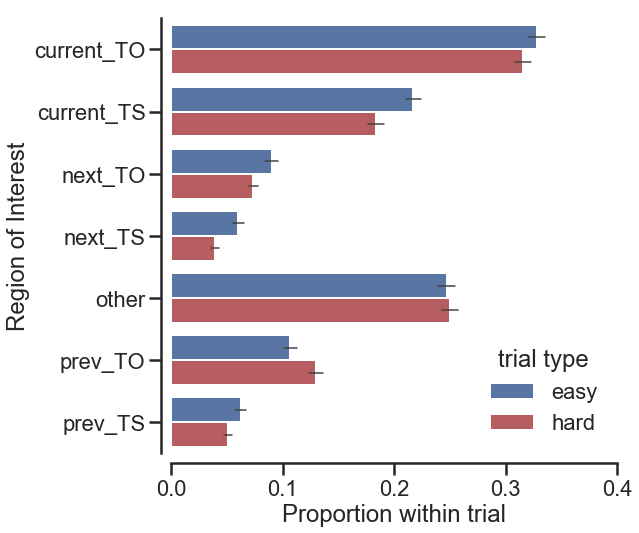
\includegraphics[width=0.3\linewidth]{source/figures/results/first_fix_roi_execution.png}\label{figure:t50_exe_fix_prop}}
    \caption[]{ T50 for the action execution epochs. In order to capture the latency T50 as an estimator for latency of first fixation on the 7 ROIs per trial. 
    Panel \protect\subref{figure:t50_sub_exe} shows the mean and 95\% confidence interval of T50 estimate for each trial. Blue points show the mean T50 for EASY trials and red points show the the T50 for the HARD trials.
    Panel \protect\subref{figure:t50_exe_fix_prop} shows the proportion of first fixations on each of the 7 ROIs. Blue bars show proportion of first fixation on given ROI for EASY trials, red bars for HARD trials. Error bars indicate 95\% confidence interval.
    }
    \label{figure:t50_subject_exe}
\end{figure}

\begin{figure}[h]
    \centering
    \subfloat[]{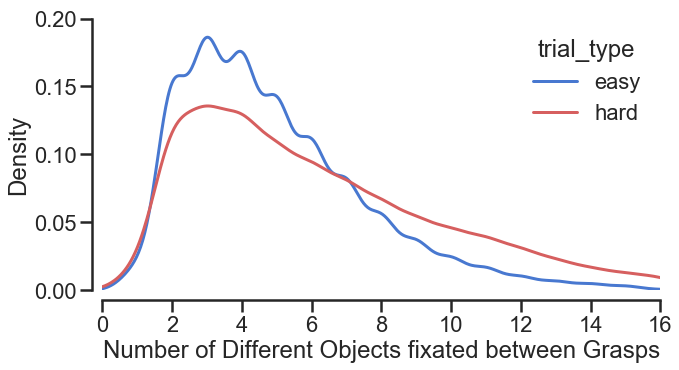
\includegraphics[width=0.5\linewidth]{source/figures/results/fixations_between_grasps.png}
    \label{figure:fix_bw_grasp}} 
    \subfloat[]{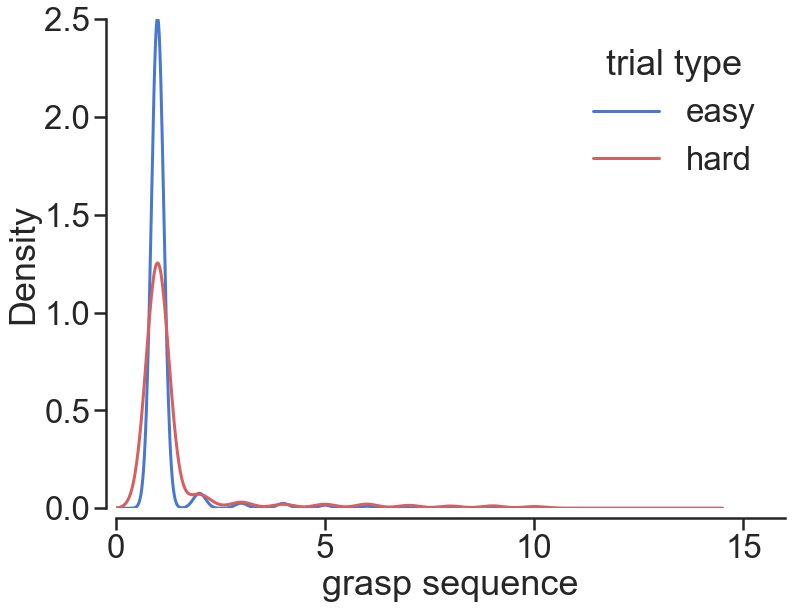
\includegraphics[width=0.4\linewidth]{source/figures/results/lookahead_distance_most_fixated.png}
    \label{figure:most_fixated}}\\
    \subfloat[]{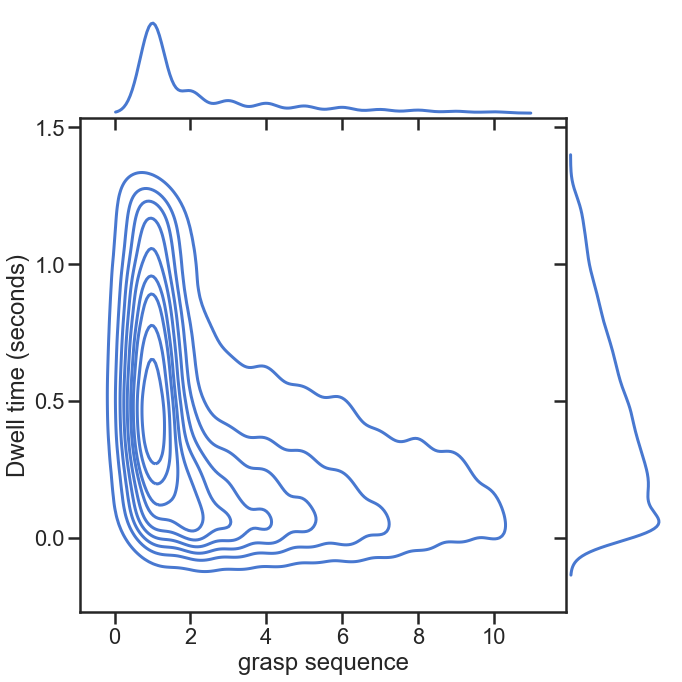
\includegraphics[width=0.4\linewidth]{source/figures/results/lookahead_distance_duration_easy.png}
    \label{figure:tla_easy}}
    \subfloat[]{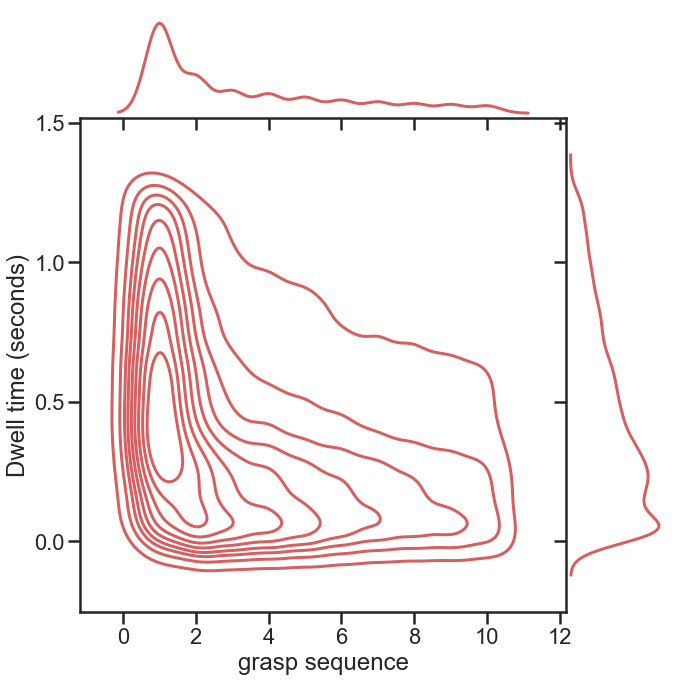
\includegraphics[width=0.4\linewidth]{source/figures/results/lookahead_distance_duration_hard.png}
    \label{figure:tla_hard}}
    \caption[]{\protect\subref{figure:fix_bw_grasp} shows the probability density of unique objects fixated on between consecutive grasps for the two trial types EASY (blue) and HARD (red). For both EASY and HARD trials, maximum probability density of fixation is on three unique objects in the scene. \protect\subref{figure:most_fixated} shows the probability density of the most fixated object in a grasp sequence. For both EASY and HARD trials, the maximum probability of density is on the object that is immediately grasped next, this shows that between two grasp onsets, maximum attention is allotted to the object that is next in line to be grasped. 
    \protect\subref{figure:tla_easy}\protect\subref{figure:tla_hard} show the joint probability density of the dwelling time (total fixation duration) on an object between consecutive grasps and it's position in the relative grasp sequence for EASY and HARD trials respectively. The figure also shows the marginal probability density of the dwelling time  on an object and it's relative position in grasp sequence. The abscissa refers to the relative grasp sequence of a fixated object i.e., when the grasp sequence of a fixated object is 1 the object is grasped next or when the grasp sequence is 2 the fixated object is grasped one after the next grasp.  the The figure shows that the dwelling time is highest on the object that is immediately next in line to be grasped. The dwelling time reduces linearly on the objects that are upcoming in the relative grasp sequence. The differences in the EASY and HARD trials can be explained by the higher number of objects fixated on between grasps in the HARD trials as shown in \protect\subref{figure:fix_bw_grasp}
    }
    \label{figure:planning_behavior}
\end{figure}


\begin{figure}[h]
    \centering
    \subfloat[]{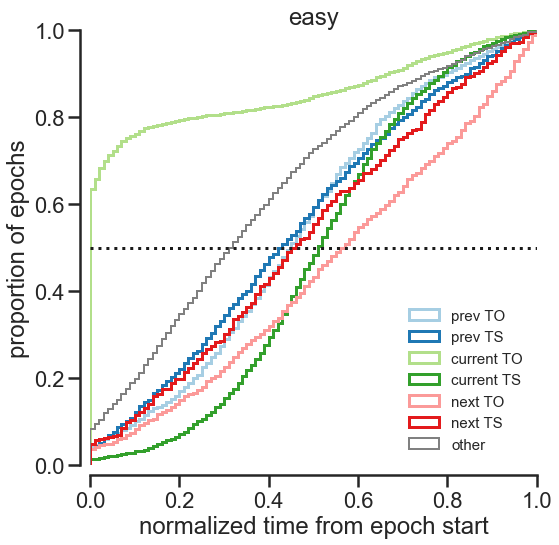
\includegraphics[width=0.3\linewidth]{source/figures/results/t50_easy_execution.png}
    \label{figure:t50_easy_exe}}
    \subfloat[]{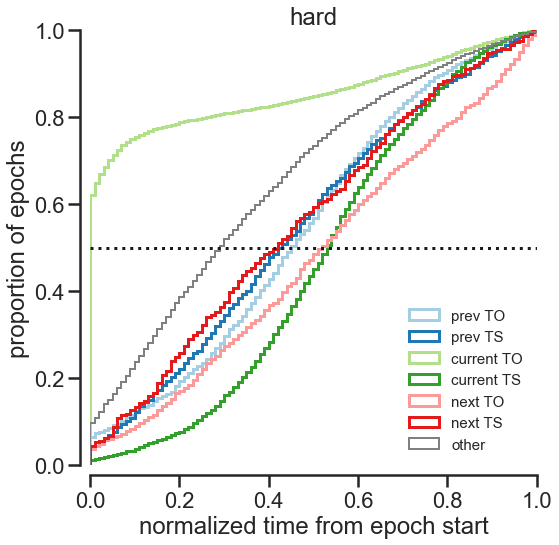
\includegraphics[width=0.3\linewidth]{source/figures/results/t50_hard_execution.png}
    \label{figure:t50_hard_exe}} \\
    \caption[]{Cumulative distributions of time of first fixation on the 7 regions of interest for the action execution epochs. The dotted line indicates time required in 50\% of all epochs to first fixation on the ROIs. The time taken for first fixation on each ROI can be  used to determine the attention attraction power of a region of interest i.e. the time taken to saccade to the region of interest.\\
    Panel \protect\subref{figure:t50_easy_exe} shows the cumulative plots for the 7 ROIs for the EASY trials. In 50\% of the action execution epochs the 7 ROIs are fixated on within half time of the epoch duration. At the 50\% mark, the curves indicate the latency of gaze shift from the current\_TO, other objects and shelves, closely followed by the previous target object and shelf (prev\_TO, prev\_TS), then to next target shelf (next\_TO), current target shelf (current\_TS) and next target object (next\_TO). This is indicative of attention equally distributed on the 6 ROIs and no selective preference for any one object or shelf in the task sequence during the later stages of action execution epoch.\\
    Panel \protect\subref{figure:t50_hard_exe} shows the cumulative distribution of the time to first fixation on the 7 ROIs for HARD trials. In 50\% of the action execution epochs, a similar trend is seen as in the EASY trials.
    }
     \label{figure:t50_overall_exe}
\end{figure}



\begin{figure}[h]
    \centering
    \subfloat[]{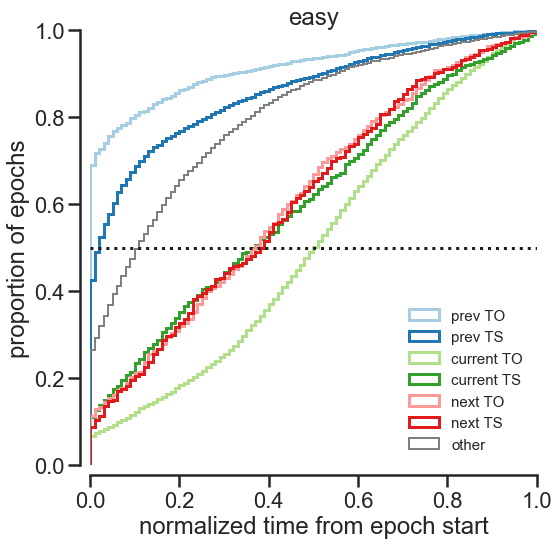
\includegraphics[width=0.25\linewidth]{source/figures/results/t50_easy_planning.png}
    \label{figure:t50_easy_plan}}
    \subfloat[]{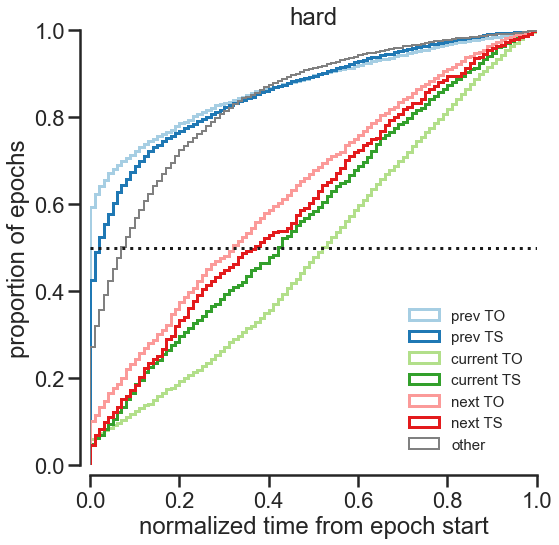
\includegraphics[width=0.25\linewidth]{source/figures/results/t50_hard_planning.png}\label{figure:t50_hard_plan}}
    \caption[]{Cumulative distributions of time of first fixation on the 7 regions of interest for action planning epoch. The dotted line indicates time required in 50\% of epochs to first fixate the ROIs.
    Panel \protect\subref{figure:t50_easy_plan} shows the cumulative plots for the 7 ROIs for the EASY trials. In 50\% of the epochs gaze is directed early to the previous target object and shelf. Further, gaze moves to other objects/shelves in the scene which is then followed by close fixations on next target object and shelf and lastly to the current target object well before the action on the object is executed. This is indicative of attention sequentially moving from one ROI to the next.
    Panel \protect\subref{figure:t50_hard_plan} shows the cumulative distribution of the time to first fixation on the 7 ROIs for HARD trials. In 50\% of the grasp epochs, The latency of first fixations on the ROIs remains roughly similar to the action planning epochs of the EASY trials, where the early fixations are on the previous target object and shelf and the last on the current target object before being manipulated.}
     \label{figure:t50_overall_plan}
\end{figure}